\documentclass[12pt]{article}

\usepackage[a4paper,margin=1in]{geometry}
\usepackage{hyperref}
\usepackage{graphicx}
\usepackage{longtable}
\usepackage{booktabs}
\usepackage{array}
\usepackage{xcolor}
\usepackage{enumitem}
\usepackage{listings}
\usepackage{caption}
\usepackage{tikz}
\usepackage{microtype}
\usetikzlibrary{positioning,arrows.meta,fit}

\newcolumntype{L}[1]{>{\raggedright\arraybackslash}p{#1}}
\newcolumntype{C}[1]{>{\centering\arraybackslash}p{#1}}

\setlength{\LTleft}{0pt}
\setlength{\LTright}{0pt}

\captionsetup{justification=raggedright,singlelinecheck=false}

\definecolor{codebg}{RGB}{248,248,248}
\lstdefinestyle{sqlstyle}{
  language=SQL,
  backgroundcolor=\color{codebg},
  basicstyle=\ttfamily\small,
  keywordstyle=\color{blue!60!black}\bfseries,
  commentstyle=\color{gray},
  stringstyle=\color{orange!60!black},
  showstringspaces=false,
  columns=fullflexible,
  frame=single,
  framerule=0pt,
  breaklines=true,
  breakatwhitespace=true,
  postbreak=\mbox{\textcolor{blue!60!black}{$\hookrightarrow$}\space}
}

\lstdefinestyle{bashstyle}{
  language=bash,
  backgroundcolor=\color{codebg},
  basicstyle=\ttfamily\small,
  keywordstyle=\color{blue!60!black}\bfseries,
  commentstyle=\color{gray},
  stringstyle=\color{orange!60!black},
  showstringspaces=false,
  columns=fullflexible,
  frame=single,
  framerule=0pt,
  breaklines=true,
  breakatwhitespace=true,
  postbreak=\mbox{\textcolor{blue!60!black}{$\hookrightarrow$}\space}
}

	itle{\textbf{Library Management System\\DBMS Mini Project Report}}
\author{Karan M\\Department of Computer Science\\\texttt{karanm6505@gmail.com} \and
        Adithya Shetty\\Department of Computer Science\\\texttt{adithyas1204@gmail.com}}
\date{28~October~2025}

\begin{document}
\maketitle
\thispagestyle{empty}

\begin{center}
\vspace{1cm}
\textbf{Problem Statement}\\[0.5\baselineskip]
Design and implement a full-stack Library Management System with persistent storage, RESTful services, and operational analytics.

\vspace{1cm}
\textbf{Institution}\\[0.5\baselineskip]
Department of Computer Science \\DBMS Mini Project 2025
\end{center}

\newpage
\tableofcontents
\newpage

\section{Abstract}
The Library Management System digitizes essential library workflows spanning user authentication, catalog management, staff administration, and borrowing logistics. A MySQL schema defines normalized entities, while a Go-based REST API orchestrates validation and business rules. A React frontend delivers responsive dashboards, CRUD forms, and metadata tooling that expose stored routines and triggers. Together, the stack streamlines day-to-day operations and provides an extensible foundation for academic deployments.

\section{User Requirement Specification (Review-1)}
\subsection{Functional Requirements}
\begin{enumerate}[label=F\arabic*]
  \item User authentication with bcrypt-protected credentials and role-based access (admin, viewer).
  \item Student registry supporting create, read, update status, and audit logging hooks.
  \item Staff directory with position tracking and activation/deactivation lifecycle.
  \item Catalog management for books, covering metadata and availability updates triggered by borrow events.
  \item Borrow lifecycle handling issue, due, return operations and enforcing borrowing caps with overdue computation.
  \item Computer lab inventory tracking allocations to students and staff.
  \item Operational dashboard summarising key aggregates for administrators.
  \item Metadata utilities to list and execute stored routines securely via the backend.
\end{enumerate}

\subsection{Non-functional Requirements}
\begin{enumerate}[label=N\arabic*]
  \item High availability through Docker Compose orchestration and automated schema bootstrap scripts.
  \item Security via hashed passwords, JWT-authenticated admin endpoints, and defensive triggers.
  \item Performance commitment of sub-200~ms latency for common read APIs under lab workloads.
  \item Maintainability with layered Go architecture (handlers, repository, models) and unit testing hooks.
  \item Portability across macOS, Linux, and Windows through containerized deployment.
\end{enumerate}

\section{Technology Stack}
\begin{longtable}{@{}L{0.32\textwidth}L{0.6\textwidth}@{}}
\toprule
\textbf{Layer} & \textbf{Technology} \\
\midrule
Database & MySQL~8.4 \\
Backend & Go~1.22, Chi router, \texttt{database/sql}, \texttt{go-sql-driver/mysql} \\
Frontend & React~18, Vite, TypeScript, Tailwind CSS \\
Tooling & Docker Compose, npm, sqlmock (testing), bcrypt hashing \\
Optional Hosting & Render / Railway-compatible containers \\
\bottomrule
\end{longtable}

\section{Entity--Relationship Diagram}
\begin{figure}[H]
  \centering
  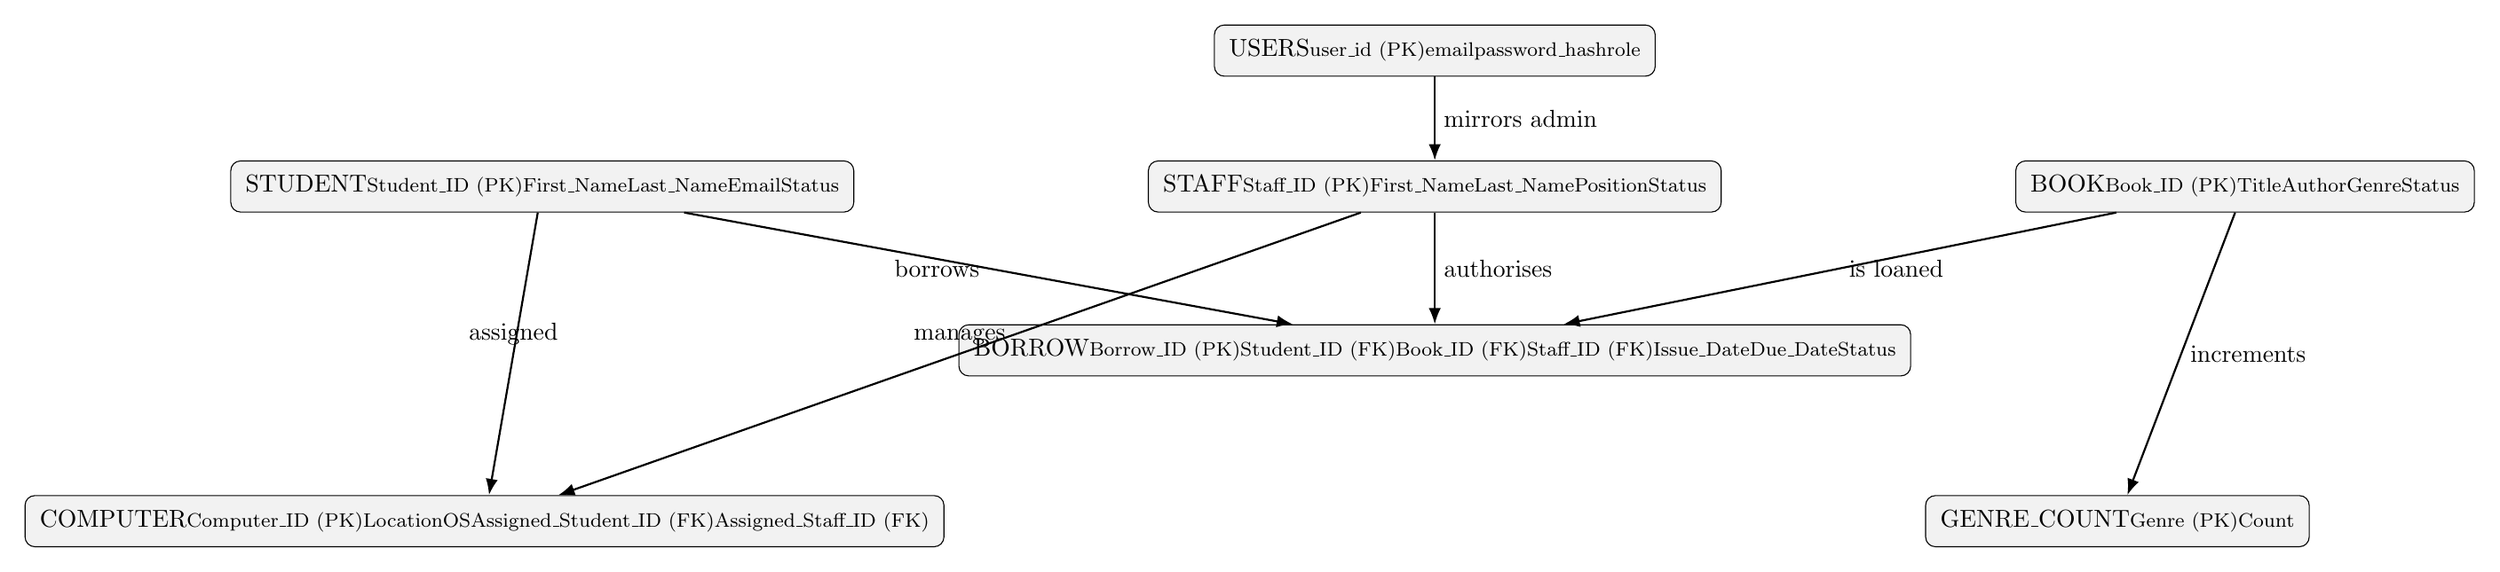
\begin{tikzpicture}[
      entity/.style={draw, rounded corners, fill=gray!10, inner sep=6pt, minimum width=3.4cm},
      rel/.style={-Latex, thick}
    ]
    \node[entity] (users) {USERS\\\footnotesize user\_id (PK)\\email\\password\_hash\\role};
    \node[entity, below=1.2cm of users] (staff) {STAFF\\\footnotesize Staff\_ID (PK)\\First\_Name\\Last\_Name\\Position\\Status};
    \node[entity, left=4.2cm of staff] (student) {STUDENT\\\footnotesize Student\_ID (PK)\\First\_Name\\Last\_Name\\Email\\Status};
    \node[entity, right=4.2cm of staff] (book) {BOOK\\\footnotesize Book\_ID (PK)\\Title\\Author\\Genre\\Status};
    \node[entity, below=1.6cm of staff] (borrow) {BORROW\\\footnotesize Borrow\_ID (PK)\\Student\_ID (FK)\\Book\_ID (FK)\\Staff\_ID (FK)\\Issue\_Date\\Due\_Date\\Status};
    \node[entity, below left=1.7cm and 0.2cm of borrow] (computer) {COMPUTER\\\footnotesize Computer\_ID (PK)\\Location\\OS\\Assigned\_Student\_ID (FK)\\Assigned\_Staff\_ID (FK)};
    \node[entity, below right=1.7cm and 0.2cm of borrow] (genre) {GENRE\_COUNT\\\footnotesize Genre (PK)\\Count};

    \draw[rel] (student) -- node[left]{borrows} (borrow);
    \draw[rel] (staff) -- node[right]{authorises} (borrow);
    \draw[rel] (book) -- node[right]{is loaned} (borrow);
    \draw[rel] (student) -- node[above]{assigned} (computer);
    \draw[rel] (staff) -- node[above]{manages} (computer);
    \draw[rel] (book) -- node[right]{increments} (genre);
    \draw[rel] (users) -- node[right]{mirrors admin} (staff);
  \end{tikzpicture}
  \caption{Entity--Relationship model of the Library Management System.}
\end{figure}

\section{Relational Schema}
\begin{longtable}{@{}L{0.18\textwidth}L{0.18\textwidth}L{0.24\textwidth}L{0.3\textwidth}@{}}
\toprule
\textbf{Table} & \textbf{Primary Key} & \textbf{Foreign Keys} & \textbf{Highlights} \\
\midrule
users & user\_id & --- & unique email, bcrypt password hash, role enum \\
student & Student\_ID & --- & active/inactive status tracking \\
staff & Staff\_ID & --- & position, status lifecycle \\
book & Book\_ID & --- & genre, publisher, availability state \\
borrow & Borrow\_ID & Student\_ID, Book\_ID, Staff\_ID & issue/due dates, status field \\
computer & Computer\_ID & Assigned\_Student\_ID, Assigned\_Staff\_ID & workstation allocation metadata \\
genre\_count & Genre & --- & maintained by triggers, aggregated counts \\
\bottomrule
\end{longtable}

\section{DDL Commands (Excerpt)}
\begin{lstlisting}[style=sqlstyle,caption={Core schema definitions}]
CREATE TABLE users (
    user_id INT AUTO_INCREMENT PRIMARY KEY,
    email VARCHAR(100) NOT NULL UNIQUE,
    password_hash VARCHAR(255) NOT NULL,
    role ENUM('admin', 'viewer') NOT NULL DEFAULT 'viewer',
    created_at TIMESTAMP DEFAULT CURRENT_TIMESTAMP,
    updated_at TIMESTAMP DEFAULT CURRENT_TIMESTAMP ON UPDATE CURRENT_TIMESTAMP
);

CREATE TABLE borrow (
    Borrow_ID INT PRIMARY KEY,
    Student_ID INT,
    Book_ID INT,
    Staff_ID INT,
    Issue_Date DATE,
    Due_Date DATE,
    Status VARCHAR(20),
    FOREIGN KEY (Student_ID) REFERENCES student(Student_ID),
    FOREIGN KEY (Book_ID) REFERENCES book(Book_ID),
    FOREIGN KEY (Staff_ID) REFERENCES staff(Staff_ID)
);

CREATE TABLE genre_count (
    Genre VARCHAR(50) PRIMARY KEY,
    Count INT NOT NULL DEFAULT 0
);
\end{lstlisting}
Full data definition and seeding statements are compiled in \texttt{docs/full\_project\_queries.sql}.

\section{CRUD Operation Evidence}
\begin{longtable}{@{}L{0.25\textwidth}L{0.38\textwidth}L{0.29\textwidth}@{}}
\toprule
Operation & Frontend Flow & Screenshot Placeholder \\
\midrule
Create Student & Dashboard \textrightarrow{} Students \textrightarrow{} ``Add Student'' modal & screenshots/student-create.png \\
Read Books & Dashboard \textrightarrow{} Books table with filters & screenshots/books-list.png \\
Update Borrow Status & Borrow detail drawer \textrightarrow{} ``Mark Returned" & screenshots/borrow-update.png \\
Delete Staff & Staff list \textrightarrow{} context menu \textrightarrow{} ``Deactivate" (logical delete) & screenshots/staff-deactivate.png \\
\bottomrule
\end{longtable}
\textit{Note: Replace placeholders with captured PNG images before submission.}

\section{Feature Showcase}
\begin{longtable}{@{}L{0.25\textwidth}L{0.38\textwidth}L{0.29\textwidth}@{}}
\toprule
Feature & Description & Screenshot Placeholder \\
\midrule
Analytics Dashboard & KPI cards displaying active counts and overdue metrics & screenshots/dashboard-overview.png \\
Metadata Explorer & UI to list/execute tables, functions, procedures, and triggers & screenshots/metadata-browser.png \\
Auth Workflow & JWT-secured login form & screenshots/login.png \\
Borrow Wizard & Guided modal for selecting student, book, and due date & screenshots/borrow-wizard.png \\
\bottomrule
\end{longtable}

\section{Database Logic Assets}
\subsection{Triggers}
\begin{enumerate}
  \item \texttt{after\_borrow\_insert} --- marks a book as \texttt{Issued} upon borrow creation.
  \item \texttt{after\_borrow\_return} --- restores a book to \texttt{Available} when status changes.
  \item \texttt{after\_book\_insert} --- increments \texttt{genre\_count} on new book entry.
  \item \texttt{before\_book\_delete} --- prevents deleting books that are loaned out.
  \item \texttt{after\_staff\_insert} --- defaults staff status to \texttt{Active} when omitted.
  \item \texttt{before\_borrow\_limit} --- enforces a three-book limit per student.
\end{enumerate}

\subsection{Stored Procedures}
\begin{itemize}
  \item \texttt{add\_new\_book} --- inserts titles with default availability.
  \item \texttt{get\_active\_staff\_list} --- returns all staff entries with status \texttt{active}.
  \item \texttt{get\_books\_borrowed\_by\_student} --- joins \texttt{book} and \texttt{borrow} to list active loans.
  \item \texttt{get\_books\_borrowed\_with\_overdue} --- surfaces overdue durations per title.
  \item \texttt{get\_currently\_borrowed\_books} --- lists currently issued books.
  \item \texttt{list\_functions}, \texttt{list\_procedures}, \texttt{list\_triggers} --- metadata introspection helpers.
\end{itemize}

\subsection{Stored Functions}
\begin{itemize}
  \item \texttt{active\_staff\_count()} --- counts active staff.
  \item \texttt{borrowed\_count(stu\_id)} --- counts active borrows per student.
  \item \texttt{is\_book\_available(bookid)} --- boolean availability check.
  \item \texttt{overdueby(due\_date)} --- calculates days past due.
  \item \texttt{total\_books\_in\_genre(genre\_name)} --- genre-based inventory aggregate.
\end{itemize}

\section{Invocation Snippets}
\subsection{REST API}
\begin{lstlisting}[style=bashstyle,caption={Executing stored routines via backend APIs}]
# Execute stored procedure (admin JWT required)
curl -X POST \
  -H "Authorization: Bearer <token>" \
  -H "Content-Type: application/json" \
  -d '{"arguments": [1]}' \
  http://localhost:5050/api/schema/procedures/get_books_borrowed_by_student/execute

# Execute stored function
curl -X POST \
  -H "Authorization: Bearer <token>" \
  -H "Content-Type: application/json" \
  -d '{"arguments": ["Artificial Intelligence"]}' \
  http://localhost:5050/api/schema/functions/total_books_in_genre/execute
\end{lstlisting}

\subsection{Direct SQL}
\begin{lstlisting}[style=sqlstyle,caption={Invoking stored routines and inspecting triggers}]
CALL add_new_book('Refactoring', 'Martin Fowler', 'Addison-Wesley', 2019, 'Programming');
SELECT total_books_in_genre('Programming');

-- Trigger demo: attempt to exceed borrow limit
INSERT INTO borrow (Borrow_ID, Student_ID, Book_ID, Staff_ID, Issue_Date, Due_Date, Status)
VALUES (11, 1, 8, 2, CURDATE(), DATE_ADD(CURDATE(), INTERVAL 14 DAY), 'Issued');
-- Expected SIGNAL: "Cannot borrow more than 3 books at a time"
\end{lstlisting}

\section{SQL Bundle}
All SQL artefacts (CREATE, INSERT, triggers, procedures, functions, nested queries, joins, and aggregations) are consolidated in \texttt{docs/full\_project\_queries.sql}. Execute this file using the MySQL client to bootstrap the database in one pass.

\section{Repository Reference}
Project source code: \href{https://github.com/karanm6505/dbms}{github.com/karanm6505/dbms}

\section*{Next Steps}
Capture high-resolution UI screenshots, extend API coverage for update/delete pathways, and publish the report artefacts through continuous integration for traceability.

\end{document}
